\documentclass[a4paper,norsk, 10pt]{article}
\usepackage[utf8]{inputenc}
\usepackage{verbatim}
\usepackage{listings}
\usepackage{graphicx}
\usepackage[norsk]{babel}
\usepackage{a4wide}
\usepackage{color}
\usepackage{amsmath}
\usepackage{float}
\usepackage{amssymb}
\usepackage[dvips]{epsfig}
\usepackage[toc,page]{appendix}
\usepackage[T1]{fontenc}
\usepackage{cite} % [2,3,4] --> [2--4]
\usepackage{shadow}
\usepackage{hyperref}
\usepackage{titling}
\usepackage{marvosym }
%\usepackage{subcaption}
\usepackage{subfig}
\usepackage[noabbrev]{cleveref}
\usepackage{cite}


\setlength{\droptitle}{-10em}   % This is your set screw

\setcounter{tocdepth}{2}

\lstset{language=c++}
\lstset{alsolanguage=[90]Fortran}
\lstset{alsolanguage=Python}
\lstset{basicstyle=\small}
\lstset{backgroundcolor=\color{white}}
\lstset{frame=single}
\lstset{stringstyle=\ttfamily}
\lstset{keywordstyle=\color{red}\bfseries}
\lstset{commentstyle=\itshape\color{blue}}
\lstset{showspaces=false}
\lstset{showstringspaces=false}
\lstset{showtabs=false}
\lstset{breaklines}
\title{AST5220, Milestone 1}
\author{Daniel Heinesen, daniehei}
\begin{document}
\maketitle

\section{Introduction}
During the next four milestones we are going to calculate the temperature of the photons of the \textit{Comic Microwave Background} \footnote{Or to be more precise, the power spectrum of the CMB}. There are many hurdles to overcome on this journey, but the first is the expansion of the space-time in which the photons exist.

The photons we are looking at lives in the same Universe as we do, and from theoretical predictions and observations we know that this Universe is expanding, and has been doing so from the start time, thought the decoupling for matter and photons and all the way to today. As the space and time the photons occupy is expanding the photons will redshift. Heuristically this is because the photons dissipates energy to overcome this expansion \emph{Look over and rewrite}. This loss of energy leads to a decrease in the photon energy and therefore a change in the wavelength towards the redder part of the spectrum \footnote{In other words longer wavelength.}. 
We need a way of quantifying this expansion, to be ables to calculate this change in temperature. We are going to do this by solving the \textit{Friedmann equation}\eqref{eq:Friedmann} to get the Hubble parameter
\begin{equation}\label{eq:H}
H = \frac{a}{\dot{a}},
\end{equation}
where $a$ is the scale factor and $\dot{a}$ its time derivative. The Hubble parameters is an observable quantity which describes the expansion of the Universe. From this we are going to calculate the \textit{Conformal Time} $\eta$, which is a convenient way of representing cosmic time in many of the equations we are going to solve in later milestones.


\section{Theory}
The main parameters we are looking for is the Hubble parameter \eqref{eq:H} $H$ and the conformal time $\eta$. From Einsteins field equation we can obtain equations for finding $H$, namely the Friedmann equations. We only need the first of these,

\begin{equation}\label{eq:Friedmann}
H = H_0 \sqrt{(\Omega_{b,0} + \Omega_{m,0})a^{-3} + (\Omega_{r,0} + \Omega_{\nu,0})a^{-4} + \Omega_{\Lambda,0}},
\end{equation}

where $\Omega_{b,0}, \Omega_{m,0}, \Omega_{r,0}, \Omega_{\nu,0}, \Omega_{\Lambda,0}$ are the \textit{Density Parameters} for respectively baryons, (cold) dark matter, neutrinos and dark energy. These parameters are given as
\begin{equation}\label{eq:Omega}
\Omega_{x,0} = \frac{\rho_{x,0}}{\rho_{crit,0}} = \rho_{crit,0}\cdot\left[\frac{3H_0^2}{8\pi G}\right]^{-1},
\end{equation}

where $\rho_{x,0}$ is the density and $\rho_{crit,0} = \frac{3H_0^2}{8\pi G}$ is the critical density. Notice that the subscript $0$ means that these are the parameters at present time. If we instead calculate the density and the critical density at a given time, we obtain the density parameter at this time as well. We are going to assume that there are no neutrinos, and set $\Omega_{nu} = 0$ for all times.

To find the $\Omega_{x}$ throughout time, we need the densities. These are gives as
\begin{equation}\label{eq:rho}
\rho_{m} = \rho_{m,0} a^{-3}, \quad \rho_{b} = \rho_{b,0} a^{-3}, \quad \rho_{4} = \rho_{4,0} a^{-4}, \quad \rho_{\Lambda} = \rho_{\Lambda,0}.
\end{equation}

Before going on to look at the conformal time, we are going to define some variables to make our life easier. First, we are not going to have \eqref{eq:Friedmann} as a function of time or the scale factor, but rather over the logarithmic scale factor $x \equiv \ln a = - \ln(1+z)$, where $z$ is the red shift. We are also going to introduce the scaled Hubble parameter $\mathcal{H} \equiv aH$.

We can now find the conformal time $\eta$. From the FRW-line element it is easy to show that one can introduce a new time variable, defines as
\begin{equation}
\frac{d\eta}{dt} = \frac{c}{a}.
\end{equation}
It can be shown that we can rewrite this in another variable
\begin{equation}
\frac{d \eta}{da} = \frac{c}{a\mathcal{H}}.
\end{equation}
Since we have introduces the time parameter $x$, we can rewrite this again
\begin{equation}\label{eq:deta/dx}
\frac{d\eta}{da} = \frac{d\eta}{dx}\frac{dx}{da} = \frac{d\eta}{dx}\frac{d \ln a}{da} = \frac{d\eta}{dx}\frac{1}{a} \Rightarrow \frac{d\eta}{dx} = \frac{c}{a\mathcal{H}}\cdot a = \frac{c}{\mathcal{H}}.
\end{equation}
This makes it easy to integrate to find $\eta$.

\section{Method}

We are going to calculate \eqref{eq:Friedmann} by saying that we are going to look at the universe from the start of the recombination, $z = 1630.4$, to the end of recombination, $z = 614.2$, and from this to today, $z = 0$. We are then going to convert these red shifts into the logarithmic scale factor, and make a grid with $200$ points during recombination and $300$ points after. With this grid we can calculate $H$ from \eqref{eq:Friedmann}.

To find the the conformal time $\eta$ we need a new grid. This time we start with a grid from $a=10^{-10}$ to $a=1$ (today), with 1000 points. To be able to integrate \eqref{eq:deta/dx} we need initial condition for $\eta$ at the start of recombination. We can do this be noting that $a\mathcal{H}(a) \rightarrow H_0\sqrt{\Omega_r}$ as $a\rightarrow 0$\emph{Cite Callin}. This means that we can make the integral from the start of time, to recombination

\begin{equation}
\eta(a=a_{recombination}) = \int_0^{a_{recombination}} \frac{c}{a\mathcal{H}}da \approx \int_0^{a_{recombination}} \frac{c}{H_0\sqrt{\Omega_r}}da = \frac{c\cdot a_{recombination}}{H_0\sqrt{\Omega_r}}.
\end{equation}

Thus we have an initial value for $\eta$. To integrate until today, we can just use a simple Euler scheme
\begin{equation}
\eta_{i+1} = \eta_i + \frac{d\eta}{dx}\cdot dx.
\end{equation}

We want to know $\eta$ at all possible time, not just the ones used here. Thus we use a \textit{spline} on the calculated dataset to find get a continuous approximation to $\eta$.

\section{Results}


\begin{figure}[ht]
     \centering
     \subfloat[][This shows the Hubble Parameter as a function of the logarithmic scale factor $x$.]{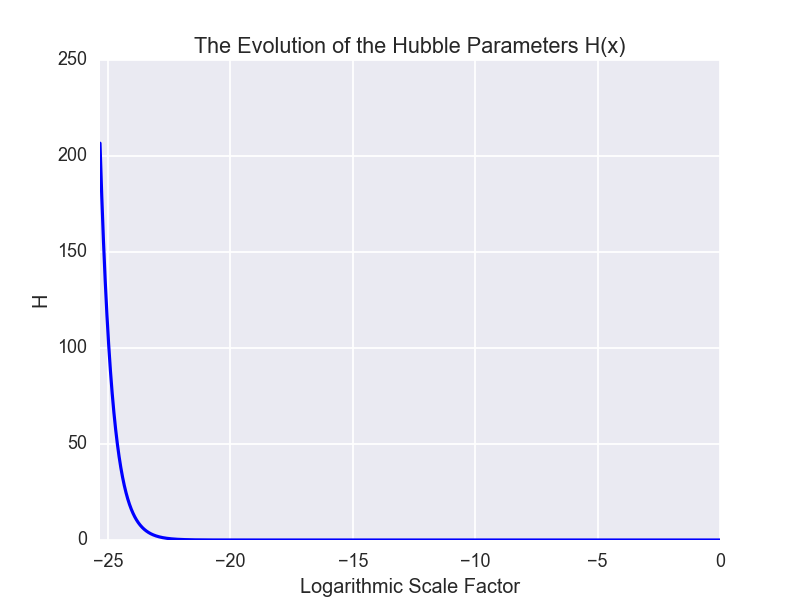
\includegraphics[scale=0.4]{H.png}\label{fig:H}}
     \subfloat[][This shows the Hubble Parameter as a function red shift $z$]{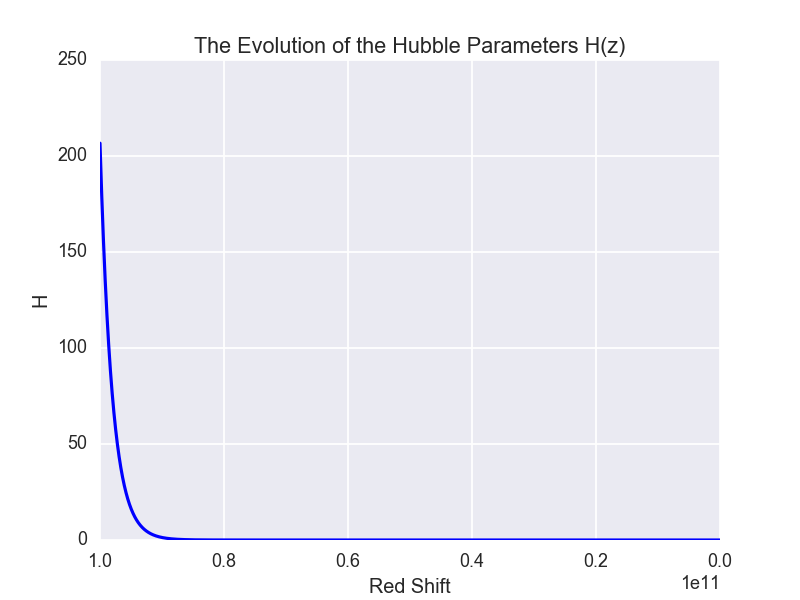
\includegraphics[scale=0.4]{H_z.png}\label{fig:H_z}}
     \caption{These plots show the evolution of the Hubble parameter through the life time of the Universe.}
     \label{fig:Hs}
\end{figure}





\end{document}


